\documentclass{beamer}
\mode<presentation> {
% The Beamer class comes with a number of default slide themes
% which change the colors and layouts of slides. Below this is a list
% of all the themes, uncomment each in turn to see what they look like.

%\usetheme{default}
%\usetheme{AnnArbor}
%\usetheme{Antibes}
%\usetheme{Bergen}
%\usetheme{Berkeley}
%\usetheme{Berlin}
%\usetheme{Boadilla}
%\usetheme{CambridgeUS}
%\usetheme{Copenhagen}
%\usetheme{Darmstadt}
%\usetheme{Dresden}
%\usetheme{Frankfurt}
%\usetheme{Goettingen}
%\usetheme{Hannover}
%\usetheme{Ilmenau}
%\usetheme{JuanLesPins}
%\usetheme{Luebeck}
\usetheme{Madrid}
%\usetheme{Malmoe}
%\usetheme{Marburg}
%\usetheme{Montpellier}
%\usetheme{PaloAlto}
%\usetheme{Pittsburgh}
%\usetheme{Rochester}
%\usetheme{Singapore}
%\usetheme{Szeged}
%\usetheme{Warsaw}
\usepackage{fancyhdr}
\usepackage{animate}
\usepackage{caption}
\usepackage{subcaption}

% As well as themes, the Beamer class has a number of color themes
% for any slide theme. Uncomment each of these in turn to see how it
% changes the colors of your current slide theme.

%\usecolortheme{albatross}
%\usecolortheme{beaver}
%\usecolortheme{beetle}
%\usecolortheme{crane}
%\usecolortheme{dolphin}
%\usecolortheme{dove}
%\usecolortheme{fly}
%\usecolortheme{lily}
%\usecolortheme{orchid}
%\usecolortheme{rose}
%\usecolortheme{seagull}
%\usecolortheme{seahorse}
%\usecolortheme{whale}
%\usecolortheme{wolverine}

%\setbeamertemplate{footline} % To remove the footer line in all slides uncomment this line
\setbeamertemplate{footline}[page number] % To replace the footer line in all slides with a simple slide count uncomment this line

\setbeamertemplate{navigation symbols}{} % To remove the navigation symbols from the bottom of all slides uncomment this line
}

\usepackage{graphicx} % Allows including images
\usepackage{booktabs} % Allows the use of \toprule, \midrule and \bottomrule in tables
\usepackage{multirow} % Allows use of multirow
%\usepackage {tikz}
\usepackage{tkz-graph}
\GraphInit[vstyle = Shade]
\tikzset{
  LabelStyle/.style = { rectangle, rounded corners, draw,
                        minimum width = 2em, fill = yellow!50,
                        text = red, font = \bfseries },
  VertexStyle/.append style = { inner sep=5pt,
                                font = \normalsize\bfseries},
  EdgeStyle/.append style = {->, bend left} }
\usetikzlibrary {positioning}
%\usepackage {xcolor}
\definecolor {processblue}{cmyk}{0.96,0,0,0}
%----------------------------------------------------------------------------------------
%	TITLE PAGE
%----------------------------------------------------------------------------------------

\title[Short title]{Particle Filter based SLAM} % The short title appears at the bottom of every slide, the full title is only on the title page

\author{Aswin P Ajayan} % Your name
\institute[Indian Institute of Technology, Bombay] % Your institution as it will appear on the bottom of every slide, may be shorthand to save space
{
Indian Institute of Technology, Bombay\\ % Your institution for the title page
\medskip
}
\date{Jun 30, 2020} % Date, can be changed to a custom date

\begin{document}

\begin{frame}
\titlepage % Print the title page as the first slide
\end{frame}

\begin{frame}
\frametitle{Overview} % Table of contents slide, comment this block out to remove it
\tableofcontents % Throughout your presentation, if you choose to use \section{} and \subsection{} commands, these will automatically be printed on this slide as an overview of your presentation
\end{frame}

%----------------------------------------------------------------------------------------
%	PRESENTATION SLIDES
%----------------------------------------------------------------------------------------

%------------------------------------------------

\section{What is SLAM}
\begin{frame}{What is SLAM}
    \begin{itemize}
    \item Computing robot's poses and map environment simultaneously \\
    \item Localisation : estimating robots location\\ 
    \item Mapping      : building a MAP\\
    \item Given
    \begin{itemize}
        \item $u_{1:T} = \{u_1,u_2,u_3....u_T\}$, the control inputs
        \item $z_{1:T} = \{z_1,z_2,z_3,...,z_T\}$, observations

    \end{itemize}
\item Wanted
    \begin{itemize}
    \item $m$, map of the environment
    \item $x_{0:T} = \{x_0,x_1,x_2,...,x_T\}$ , robot location
    \item $p(x_{0:T},m | u_{0:T},z_{1:T})$, the SLAM posterior
        \end{itemize}
\end{itemize}


\end{frame}


\section{Objective}
\begin{frame}{Objective}
    \begin{itemize}
        \item To review the literature available on SLAM. To get acquainted with various techniques available for SLAM and examine some of them in depth. Simulation in reallife constraints using ROS.\\
            Types of SLAM techniques explored includes
        \item \textbf{Kalman Filter based approaches}
            \begin{itemize}
                \item Extended Kalman Filter
                \item Unscented Kalman Filter
                \item Extended Information Filter
            \end{itemize}
            \item \textbf{Particle Filter based approaches}
                \begin{itemize}
                    \item Fast SLAM -Rao Blackwellised Particle Filter
                        \begin{itemize}
                            \item Augmented MCL
                            \item Mixture MCL
                        \end{itemize}
                \end{itemize}
       \end{itemize}
\vfill
\end{frame}


\section{Types of SLAM}
\begin{frame}{Types of SLAM}
    \begin{itemize}
        \item Full SLAM vs online SLAM
        \begin{itemize}
            \item Full SLAM $p(x_{0:T},m|u_{1:t},z_{1:t})$
            \item Full SLAM $p(x_{t},m|u_{1:t},z_{1:t})$
        \end{itemize}
        \item Feature Based SLAM vs Grid Based
\begin{figure}
     \centering
        \begin{subfigure}[b]{0.4\textwidth}
        % \centering
        \hspace*{-10mm}
        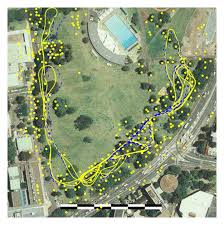
\includegraphics[height = 40mm,width = 60mm]{feature_maps.jpeg}
        \end{subfigure}
    ~
        \begin{subfigure}[b]{0.4\textwidth}
        \centering
        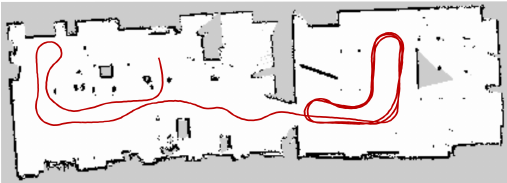
\includegraphics[height = 40mm,width = 60mm]{gridMap.png}
        \end{subfigure}
    \end{figure}   

        \item Active SLAM vs Passive SLAM
    \end{itemize}
\end{frame}


\section{Markov assumption and Recursive Bayesian estimate}
\begin{frame}{Recursive Bayesian Estimation}
    \begin{itemize} 
        \item \textbf{Markov assumption} : next state depends only on the present state
            $$p(x_{t}|x_{0:t},u_{1:t}) = p(x_t | x_{t-1},u{t})$$
        \item \textbf{Recursive Bayesian Estimation}
\begin{align*}  
    bel(x_t) & = p(x_t | z_{1:t},u_{1:t})\\
    & = \eta p(z_t|x_t) \int_{x_{t-1}} p(x_t |x_{t-1},u_t) * bel(x_{t-1})dx_{t-1}
 \end{align*}
 we can split this into predict and update steps where\\
 \textbf{Predict Step} 
 $$\overline{bel(x_t)} =  \int_{x_{t-1}} p(x_t |x_{t-1},u_t) * bel(x_{t-1})dx_{t-1}$$
 \textbf{Update Step} 
 $$bel(x_t) =  \eta * p(z_t | x_t) * \overline{bel(x_t)}$$


 \textbf{Bayes filter} recursive estimation is realised using kalman filter, Information Filter, particle filter etc.
    \end{itemize}
\end{frame}

\section{Frameworks for recursive filter estimation}
\begin{frame}{Kalman Filter Family}
    Beliefs are represented in parametric form 
    with mean vector $\mu_t$ and covariance matrix $\Sigma _t$ . Closed form expressions are available for belief propagation under certain cases

    \begin{itemize}        
        \item \textbf{Kalman Filter :} Assumes linear models(state transistion and measurement) and gaussian posterior
        \item \textbf{Extended Kalman Filter :} Linearises the model and then applies normal KF
        \item \textbf{Unscented Kalman Filter :} Samples a gaussian posterior from the resulting non linear transformation
        \item \textbf{Information Filters :} Uses canonical representaion of Belief i.e. $\mu_{t}^{-1}$ and $\Sigma_{t}^{-1}$
    \end{itemize}
\end{frame}


\section{Particle Filters}
\begin{frame}{Particle Filter}
    \begin{itemize}
        \item Use particles to represent instead of parametric models.
        \item Can effectively model mutli modal distributions . 
        \item Can Take care of the non linearities in the model  
        \item Computationally intensive
        \item Based on importance sampling principal 
    \end{itemize}
\end{frame}


\begin{frame}{Particle filter}
    \textbf{Importance Sampling} - Use to generate samples from an arbitrary distribution\\
    \begin{figure}
        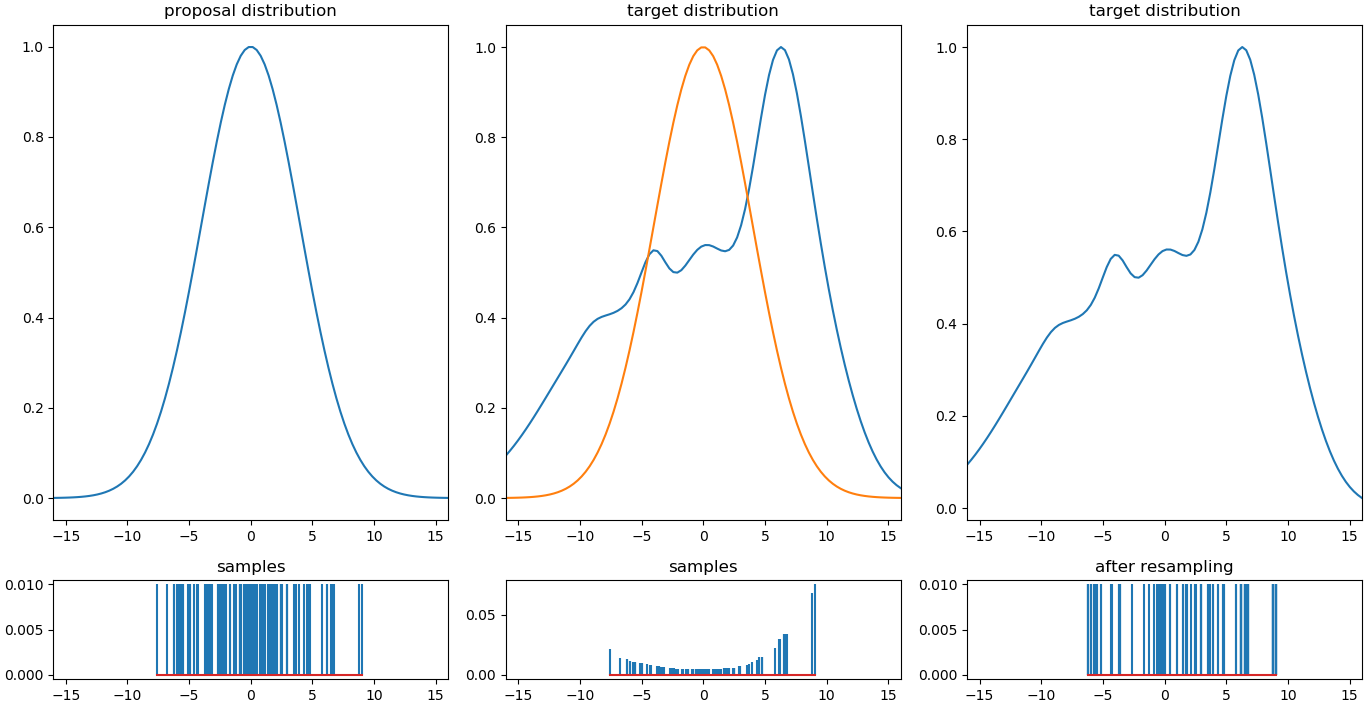
\includegraphics[height = 30mm, width = 80mm]{./importance_sampling.png}
    \end{figure}
    \textit{steps}
    \begin{itemize}
        \item Draw samples from a proposal distribution
        \item calculate the importance weight as $ w_t^{[j]} = \frac{target(x_t^{[j]})}{proposal(x_t^{[j]})}$
        \item Resample based on weights
    \end{itemize}
\tiny{$^{4}$} https://github.com/aswinpajayan/seminar-related/scripts/importance sampling.py
\end{frame}


\begin{frame}{Particle filter}
            \begin{itemize}
                \item sampling from proposal distribution : 
                    $$x_t^{[j]} \sim \pi(x_t|x_{t-1},u_{t-1})$$
                \item Importance weighting :
                    $$ w_t^{[j]} = \frac{target(x_t^{[j]})}{proposal(x_t^{[j]})} = p(z_t|x_t) $$
                \item Resampling : Draw sample $i$ with probability $w_t^{[j]}$
            \end{itemize}

\tiny{$^{1}$} Source: Probabilistic Robotics, Sebastian Thrun
\end{frame}

\section{RBPF}
\begin{frame}{Rao-Blackwellisation for SLAM - Fast SLAM 1.0}
    \begin{itemize}
        \item Particle filters are ideal for low dimensional states i.e. $|| x_t ||$ is small.
        \item for SLAM problem, Number of landmarks may be very large. So Particle filter cant be used directly
        \item Estimate the pose using particle filter and then compute map. 
\begin{align*}
    p(a,b) & = p(b|a).p(a)\\
    \sim p(x_{0:t},m_{1:M}|z_{1:t},u_{1:t}) & =  p(x_{0:t}|z_{1:t},u_{1:t}).p(m_{1:M}|z_{1:t},u_{1:t})\\
    & =  p(x_{0:t}|z_{1:t},u_{1:t}) \Pi p(m_{i}|z_{1:t},u_{1:t})\\
\end{align*}
Now each particle respresents a path hypothesis and it has an assosicated map with it. Splitting $p(m_{1:M})$ into $\Pi p(m_i)$ reduces the computational complexity further, each of this is calculated by a 2x2 EKF. 
\newline 
    \end{itemize}
\end{frame}


\begin{frame}{RBPF particle structure}
    Each particle maintains M 2x2 EKF along with the 3 pose variables 
\begin{figure}
    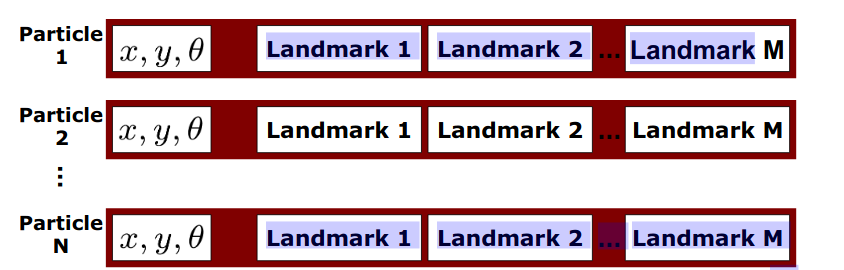
\includegraphics[width = \linewidth]{./RBPF_particles.png}
    \caption{Particle structure in RBPF-slam}
\end{figure}

\end{frame}

\section{Implementing Particle filter localisation}
\begin{frame}{Implementing Particle filter localisation}
    \begin{itemize}
        \item \textbf{Simulation Platform: } - ROS melodic Ubuntu 18.04 
        \item \textbf{Robot: } - Custom robot using URDF
        \begin{itemize}
            \item motion model libgazebo\_ros\_diff\_drive.so 
            \item sensor model head\_hokuyo\_sensor
        \end{itemize}
        \item \textbf{Visualisation: } - matplot lib interactive plots , python 2.7
    \end{itemize}
\end{frame}

\subsection{Creating a custom robot}
\begin{frame}{Creating a custom robot}
    \begin{figure}
        \centering
        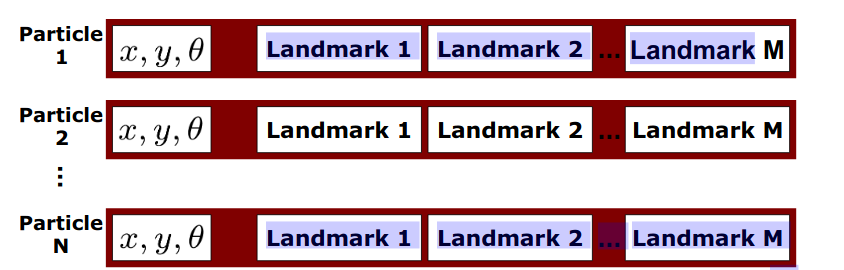
\includegraphics[width=\textwidth]{RBPF_particles.png}$^{6}$
    \end{figure}
    \begin{itemize}
    \item \textit{Universal Robot Description Format} provides an easy way to create a custom meshes for a robot. The motion model and sensor model are realised using the gazebo plugins. The robot was created using xacro files: which stands for XML Macros. 
    \item sensor: Laser range finder with standard deviation 0.01 and gaussian model was used
    \end{itemize}
    \vfill
    \tiny{$^{3}$} Source: theconstructsim.com
\end{frame}

\subsection{Creating a motion model}
\begin{frame}{Creating a motion model}
    \begin{itemize}
        \item Particle filter uses a motion model as the proposal distribution and sensor model for inferring importance weights 
        \item  A simple motion model was used :\\
            $$x_t = x_{t-1} + v.cos(\theta_{t-1})$$
            $$y_t = y_{t-1} + v.sin(\theta_{t-1})$$
            $$\theta _t = \theta _{t-1} + w \delta _{t}$$
        v, w are linear velocity, angular velocity. 
    \end{itemize}
\end{frame}

\subsection{creating a sensor model}
\begin{frame}{Creating a sensor model}
    \begin{itemize}

        \item Maximum likelihood field was chosen to be used as the sensor model 
        \item The field was generated using a convolution with a kernel and point landmark map.
\begin{figure}


     \centering
        \begin{subfigure}[b]{0.4\textwidth}
        % \centering
        \hspace*{-10mm}
        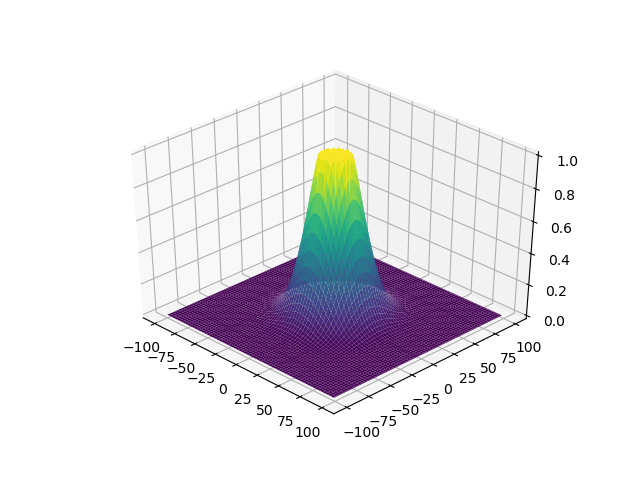
\includegraphics[height = 40mm,width = 60mm]{kernel.png}
        \end{subfigure}
    ~
        \begin{subfigure}[b]{0.4\textwidth}
        \centering
        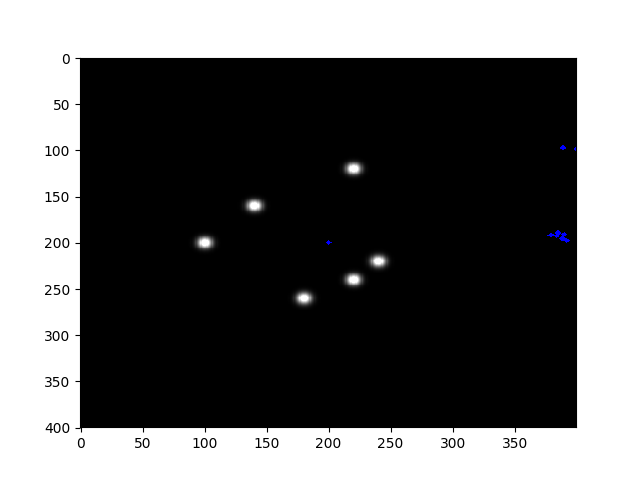
\includegraphics[height = 40mm,width = 60mm]{ML field.png}
        \end{subfigure}
    \end{figure}   


    \end{itemize}
\end{frame}


\subsection{Resampling}
\begin{frame}{Resampling}
    Various Resampling approaches were tried out -
    \begin{itemize}
        \item \textbf{Fitness proportion sampling:} Used the default resampler available in numpy \\
            \textit{numpy.random.choice(particles, num=N, p=weights)}
        \item \textbf{Roulette wheel selection :} Fitnesss values arranged as CDF around a wheel and a point is chosen at random
        \item \textbf{Stochastic Universal sampling :} Roulette wheel selection will be dominated by a few particles of highest fit. Some particles with high fitness values might be shadowed by the most fit members. This can result is global localisation failure. To avoid this SUS was tried. Though it reduces localisation failure, it can still result in localisation failure  
    \end{itemize}
\end{frame}

\section{Simulations}
\begin{frame}{Simulations}
    \begin{figure}
        \centering
        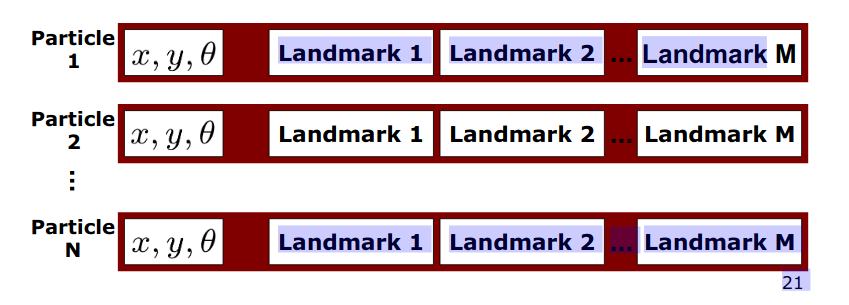
\includegraphics[width=\textwidth]{RBPF_SLAM.png}$^{7}$
    \end{figure}
\end{frame}


% \begin{frame}{DLC384 Reading FSM Diagram}
%      \begin{figure}
%         \includegraphics[width = 100mm]{DLC384-reading-FSM.png}$^{8}$
%     \end{figure}   
% \end{frame}


\begin{frame}{Analysis of DLC384 Reading FSM Diagram and clock diagram from data sheet}
     \begin{figure}
     \centering
        \begin{subfigure}[b]{0.4\textwidth}
        % \centering
        \hspace*{-10mm}
        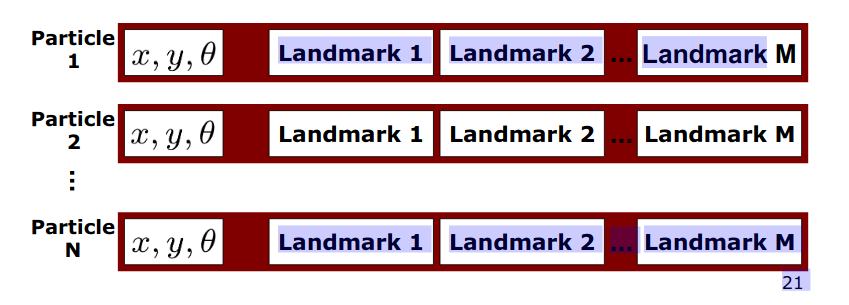
\includegraphics[height = 60mm,width = 60mm]{RBPF_SLAM.png}
        \end{subfigure}
    ~
        \begin{subfigure}[b]{0.4\textwidth}
        \centering
        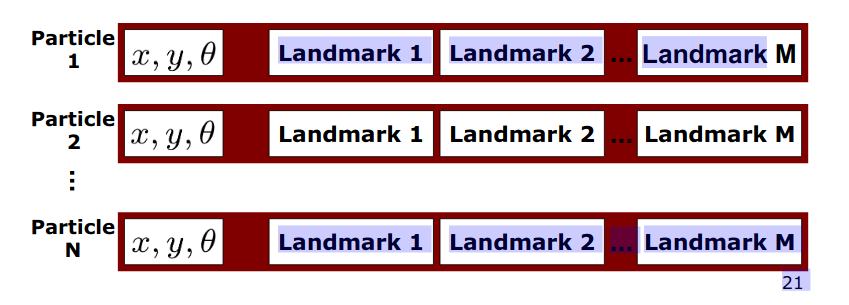
\includegraphics[height = 60mm,width = 60mm]{RBPF_SLAM.png}$^{8}$
        \end{subfigure}
    \end{figure}   
\end{frame}


\begin{frame}{DLC384 Reading FSM}
     \begin{itemize}
         \item DLC384 Reading FSM is a finite state machine having 4 states, a) State\_Reset; b) State\_INT; c) State\_EN; d) State\_Read.
         \item States (c) and (d) are two main states, in which FSM toggle’s maximum amount of time.
         \item In state (C) FSM waits for “VOUT\_EN” signal from DLC384 which is expected to arrive after 18.5 cycles from “INT” falling edge.
         \item In State (d) “INT” signal is high( for 384 cycles) so that integration of next row pixels can be done. Also since VOUT\_EN is high so simultaneously current row’s pixels value is captured at every rising edge of clock.
     \end{itemize}
\end{frame}


\begin{frame}{DLC384 Controller FSM Diagram}
    \begin{figure}
        \centering
        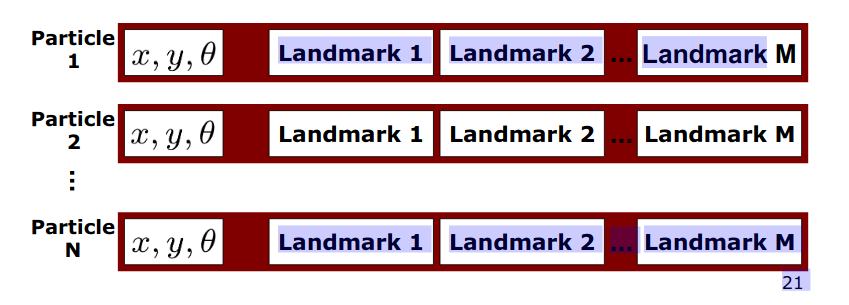
\includegraphics[width=\textwidth]{RBPF_SLAM.png}$^{9}$
    \end{figure}
\end{frame}


\begin{frame}{DLC384 Controller}
    \begin{itemize}
        \item There are two different input pins used to configure this sensor, SERIAL and SERDAT.
        \item If SERIAL = 0V then SERDAT is off and CTIA capacitance (on which integration charge accumulates) is fixed to 14 pF.
        \item If SERIAL = 5 V and SERDAT = 0V then CTIA capacitance is fixed to 18 pF or by sending some bit streams via SERDAT pin we can set different CTIA capacitance and different functions of the sensor can also be changed like(HFLIP,VFLIP).
        \item As can be seen in FSM diagram of the DLC384 controller, which transmit 51 bits from SERDAT pin if SERIAL pin is high.
        \item SERIAL pin is connected to DIP pin of FPGA board which can be turn on/off externally.
        \item Bit streams are hardcoded in FPGA which can be later controlled from DIP switches.
    \end{itemize}
\end{frame}


\section{Pin Configuration}
\begin{frame}{Pin Configuration and it's Key Number}
    \begin{table}[]
        \centering
        \resizebox{\textwidth}{!}{\begin{tabular}{|c|c|c|c|c|c|}
            \hline
            \textbf{In Port} & \textbf{Pin} & \textbf{Key} & \textbf{Out Port} & \textbf{Pin} & \textbf{Key} \\
            \hline
             resetn & j15 & Key0 & reset\_out & PIN\_A2 & GPIO\_02 \\
            \hline
            inclk & R8 & 50 MHz osc & int & PIN\_A3 & GPIO\_03 \\
            \hline
            vout\_en & PIN\_D3 & GPIO\_00 & clock\_6.25 & PIN\_B3 & GPIO\_04 \\
            \hline
            fr & PIN\_C3 & GPIO\_01 & pll\_locked & PIN\_A15 & LED0 \\
            \hline
              \multirow{2}{*}{Vout\_ADC} & PIN\_A4,B5,A5, & GPIO\_06 & serial\_out & PIN\_B4 & GPIO\_05 \\
              \cline{4-6} 
             & D5,B6,A6,B7,D6 & to GPIO\_013 & serdat & PIN\_A4 & GPIO\_06 \\
            \hline
            \end{tabular}}
        \caption{1}
    \end{table}
\end{frame}


\section{FPGA Resources Used}
\begin{frame}{Resources Used}
    \begin{table}[]
        \centering
        \resizebox{\textwidth}{!}{\begin{tabular}{|c|c|}
            \hline
            \textbf{Resource Name} & \textbf{Number/\% used} \\
            \hline
             Total Logic Elements & 153/22320 (less than 1\%)\\
            \hline
            Total Registers & 44 \\
            \hline
            Total Memory Bits & 524288/608256 (86\%) \\
            \hline
            Total PLLs & 1/4 (25\%) \\
            \hline
            
            \end{tabular}}
        \caption{2}
    \end{table}
\end{frame}



\section{Simulation Results}
\begin{frame}{Simulation Results Part-1: Control Signal analysis}
    \begin{figure}
        \centering
        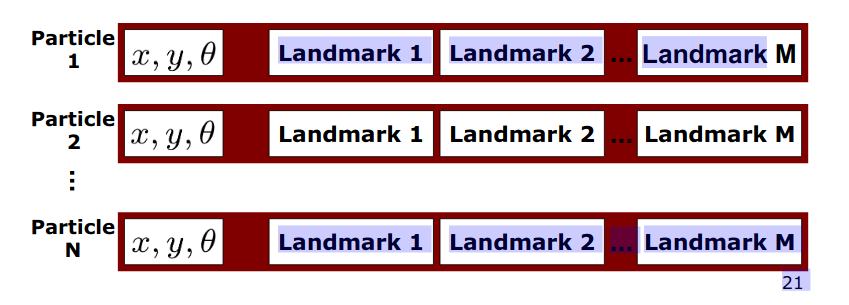
\includegraphics[width=\textwidth]{RBPF_SLAM.png}$^{10}$
    \end{figure}
\end{frame}


\begin{frame}{Simulation Results Part-1: Control Signal analysis}
    \begin{itemize}
        \item To compare the simulated timing pulses of control signals with data sheet of DLC384 it is assumed that in a frame -
            \begin{itemize}
                \item Number of columns are 5, in place of 384.
                \item Number of Rows are 3, in place of 288.
                \item Number of cycles after which the next row is read (VOUT\_EN is asserted to ‘1’ after INT is asserted to ‘0”) is 2.5 in place of 18.5.
            \end{itemize}
        \item Simulation timing pulses of control signals (figure-10) and Clock Diagram of DLC384 (figure-6) overlaps.
        \item we can calculate the pulse duration by looking at following counter values (In Figure-10).
            \begin{itemize}
                \item For 2.5 cycle(for sensor it is 18.5), for which “VOUT\_EN” is low, look for “q\_18\_cycle”.
                \item For 5 cycle(for sensor it is 384), for which “VOUT\_EN” and “INT” are high, look for “s\_h\_counter”.
                \item For current “s\_v\_count” to be seen.
            \end{itemize}
    \end{itemize}
\end{frame}


\begin{frame}{Simulation Results Part-1: Control Signal analysis (continue)}
    \begin{itemize}
        \item Using “s\_v\_count” and “s\_h\_count” values current pixel location/index can be calculated.
        \item For reset, look for “s\_reset\_out”.
        \item 6.25 MHz clock is “s\_clock\_6\_out”.
        \item Signal “fr” marks the start of a new frame, after reset is done.
        \item If "s\_serial" is high then "s\_serial\_out" is set to high and at "s\_serdat" configuration bits are sent.
    \end{itemize}
\end{frame}



\begin{frame}{Simulation Results Part-2: Working on actual images stored in a text file}
    \begin{itemize}
        \item 3 images of same pixel size is taken, considered as 3 consecutive frames of a
video.(img\_1.png, img\_2.png, img\_3.png)
        \item Using a python script, images are converted into a single vector and then saved
in a file one after another. This file will simulate the camera pixels.(Python script -
image\_to\_text.ipynb , file - img\_1\_2\_3.txt)
        \item In Quartus, a test bench is created which simulates the Camera sensor DLC384
sensor and read file “img\_1\_2\_.txt” for throwing pixels value.
        \item Sensor DLC384 gives analog value at VOUT pin, so a ADC considered b/w the
sensor and the camera driver.
        \item Once a frame is sent, testbench reads the Dual Port RAM and saves the data in
another file “output\_img.txt”.
        \item After the simulation both “img\_1\_2\_3.txt” and “out\_img.txt” files are compared
using a python script, which shows both matches perfectly.
    \end{itemize}
\end{frame}

\begin{frame}{Simulation Results Part-3: DLC384 Controller}
    \begin{itemize}
        \item DLC384 Controller simulation can be seen in figure-10, where “s\_serial\_out” and
s\_serdat” should be connected to “SERIAL” and “SERDAT” pins of the DLC384 sensor.
    \end{itemize}
\end{frame}


\section{Future Work}
\begin{frame}{Future Work}
\begin{itemize}
    \item Built an interface between Dual Port RAM(ping\_pong concept can also be introduced) and VGA port, so the video can be observed on a VGA ,monitor.
    \item DeO-Nano development board give 3.3 V as high and 0V as low, but Sensor pins works at 5V(as high) and 0V(as low) so level-shifter circuit need to be used.
\end{itemize}
\end{frame}

\section{References}
\begin{frame}{References}
\begin{thebibliography}{}
\setbeamertemplate{bibliography item}[text]
\bibitem{1} https://www.opli.net/opli\_magazine/imaging/2017/sierra-olympic-introduces-world-first-true-hd-thermal-camera-jan-news/
\bibitem{2} https://in.element14.com/terasic-technologies/p0082/e22f17c6n-DEO-nano-dev-kit/dp/2076463
\bibitem{3} http://www.123-cctv.com/CCTV-Monitors/7-inch-Security-LCD-Monitor-with-VGA.html
\bibitem{4} DLC384 User Manual
\bibitem{5} A Design of Readout Circuit for 384x288 Uncooled Microbolometer Infrared Focal Plane Array - 2012 IEEE 11th International Conference on Solid-State and Integrated Circuit
\bibitem{6} Large dynamic range Readout Integrated Circuit for Infrared Detectors -2019 32nd International Conference on VLSI Design and 2019 18th International Conference on Embedded Systems (VLSID)
\end{thebibliography}
\end{frame}


\begin{frame}
\Huge{\centerline{Thank You for your Attention}}
\end{frame}

\end{document}
